\documentclass{article}
\usepackage[utf8]{inputenc}
\usepackage[T1]{fontenc}
\usepackage[french]{babel}
\usepackage{graphicx}
\usepackage{siunitx}
\usepackage{array}
\usepackage[a4paper, total={6in, 8in}]{geometry}
\usepackage{longtable}

\setlength{\tabcolsep}{5pt}
\renewcommand{\arraystretch}{1.5}

\begin{document}

\begin{titlepage}
\newcommand{\HRule}{\rule{\linewidth}{0.5mm}} 
\center


\includegraphics[width=6cm]{assets/logo_unamur}
\\[2cm]

\textsc{\LARGE Université de Namur}
\\[2cm]

\textsc{\Large IDASM103 : Visualisation de l'information}
\\[0.2cm]

\HRule
\\[0.4cm]
\textsc{\huge Pimp My Requin}
\\[0.2cm]
\HRule
\\[0.4cm]
{\large 2023 - 2024}

\begin{figure}[h!]
	\centering
	\includegraphics[width=7cm]{assets/logo_pimpmyrequin}
    \\[0.7cm]
\end{figure}

\begin{minipage}{0.5\textwidth}
	\begin{flushleft} 
		\emph{Auteur}
		\\
		\textsc{Lambois} Emeric
		\\
		\textsc{Mernier} Julien
		\\
		\textsc{Pans} Benjamin
		\\
		\textsc{Santelé} Victor
		\\
		\textsc{Smith} Jonathan
		\\
	\end{flushleft}
\end{minipage}
~
\begin{minipage}{0.4\textwidth}
	\begin{flushright}
		\emph{Professeur}
		\\
		\textsc{Clarinval} Antoine
		\\
	\end{flushright}
\end{minipage}

\end{titlepage}

\newpage

\tableofcontents

\clearpage
\section{Introduction}

Dans le cadre du cours de « Visualisation de l’information », nous avons été chargés de concevoir un outil de visualisation répondant aux besoins d’un utilisateur choisi. Effectivement, la créativité octroyée lors de ce projet, nous autorise à choisir l’utilisateur cible que nous voulons, ainsi que l’objectif de notre outil de visualisation. Cependant, cet outil devait porter sur le jeu de données mis à disposition, qui décrivait des attaques de requins.
De ce fait, nous avons saisi l’opportunité créative que l’on nous a laissée et réfléchit sur le thème imposé. Ce qui nous a conduit à imaginer un outil de visualisation servant de configurateur de requin, avec pour objectif de pouvoir recréer un mégalodon si on le souhaite en prenant les particularités de divers requins ayant réalisé des attaques sur les humains.

\clearpage
\section{Abstraction des données}

Dans cette partie, nous allons détailler la démarche et la méthodologie que nous avons adopté dans le but d’obtenir un dataset pratique et simple d’utilisation. Nous allons tout d’abord aborder le jeu de données qui était mis à disposition et le détailler. Ensuite, nous allons détailler notre démarche de nettoyage de données pour obtenir notre dataset utilisable. Enfin, nous détaillerons les informations concernant notre jeu de données final.

\subsection{Dataset initial}

Le jeu de données mis à disposition recensait 6448 attaques de requins, avec pour chaque attaque 23 features communiquant des informations sur celle-ci. Dans les informations se trouvant dans le jeu de données, nous pouvons par exemple retrouver pour chaque attaque de requins, la date à laquelle s’est déroulé celle-ci, le pays où l’attaque s’est réalisée, la position géographique (Latitude, Longitude), l’espèce de requin, etc.
Parmi ces 23 features, nous avons décidé de seulement se focaliser sur certaines, car elles se révélaient pertinentes pour ce que nous voulions faire avec notre outil de visualisation.
C’est pourquoi, nous avons choisi d’utiliser :


\begin{table}[h]
\centering
\begin{tabular}{|m{1.9cm}|m{4cm}|m{3.3cm}|m{3.5cm}|}
\hline
Attributs & Description & Type de données & Informations complémentaires (?) \\ \hline
Espèce de requin («Species») & Décrit l’appartenance ou les propriétés physiques du requin qui a réalisé l’attaque. & Données catégorielles & 1576 espèces uniques \\ \hline
Latitude & Latitude de l’attaque observée & Données divergentes & Descend jusque \ang{-180}, monte jusque \ang{180}, avec \ang{0} comme point central \\ \hline
Longitude & Longitude de l’attaque observée & Données divergentes & Descend jusque \ang{-180}, monte jusque \ang{180}, avec \ang{0} comme point central \\ \hline
Position & La position de l’attaque observée est obtenue grâce à sa latitude et sa longitude. & Données divergentes & Descend jusque \ang{-180} \ang{-180}, monte jusque \ang{180} \ang{180}, avec \ang{0} \ang{0} comme point central \\ \hline
\end{tabular}
\end{table}

\clearpage
\subsection{Nettoyage des données}
Après avoir présenté le jeu de données initial ainsi que les attributs pertinents pour notre outil, cette section se concentrera sur les étapes de nettoyage des données que nous avons effectuées pour parvenir à notre jeu de données final.

Notre premier objectif, pour obtenir un jeu de donnée plus propre était de nettoyer l’attribut « Espèces de requins (« Species ») », cet attribut comportait 1 576 espèces uniques pour 6 448 attaques de requins. 
C’est pourquoi, nous avons tout d’abord supprimé les attaques de requins qui ne comportaient aucune espèce dans leurs informations. Cela a réduit le nombre d’attaques de requins de 6 448 à 3 302 attaques. 
Ensuite, nous avons procédé au nettoyage des noms d’espèce en supprimant les espèces n’étant pas un nom d’espèces précis. Donc les informations telles que la taille ou le poids ne nous intéressaient pas. 
De plus, certains noms d’espèce possédaient des adjectifs qui agrandissaient le nombre d’espèces différentes, alors nous avons décidé de retirer ces adjectifs pour garder exclusivement les noms d’espèces. 
Ce nettoyage a réduit considérablement les nombres d’attaques de requins donnant 1 975 attaques.
En accord avec notre objectif d’outil de visualisation, il nous manquait des informations telles que les tailles de différents attributs des requins. C’est pourquoi nous les avons générés aléatoirement via une tranche minimales et maximales pour chacun des attributs. Les tranches minimales et maximales ont été déterminés par ce que l'on a trouvé avec nos recherches.


\subsection{Jeu de données final}
Maintenant, que le nettoyage a été effectué, nous obtenons notre jeu de données final qui nous servira dans notre outil de visualisation.

\begin{longtable}[h]{|p{.25\textwidth} | p{.20\textwidth}|p{.15\textwidth}|p{.25\textwidth}|}
\hline
Attributs & Description & Type de données & Informations complémentaires (?) \\ \hline
 Espèce de requin (« Species ») & Décrit l’appartenance ou les propriétés physiques du requin qui a réalisé l’attaque. & Données catégorielles & 88 espèces uniques \\ \hline
 Latitude  & Latitude de l’attaque observée & Données divergentes  & Descend jusque -\ang{180}, monte jusque \ang{180}, avec \ang{0} comme point central  \\ \hline
 Longitude & Longitude de l’attaque observée & Données divergentes  & Descend jusque -\ang{180}, monte jusque \ang{180}, avec \ang{0} comme point central \\ \hline
 Position & La position de l’attaque observée est obtenue grâce à sa latitude et sa longitude. & Données divergentes  & 
 Descend jusque -\ang{180} -\ang{180}, monte jusque \ang{180} \ang{180}, avec \ang{0} \ang{0} comme point central \\ \hline
 Taille œil («nez\_taille\_oeil »)  & Taille de l’œil du requin & Données séquentielles & Entre 1 centimètre minimums et 10 centimètres maximum. \\ \hline
 Longueur museau (« nez\_longueur\_museau ») & Longueur du museau du requin & Données séquentielles & Entre 5 centimètres minimums et 15 centimètres maximum. \\ \hline
 Largeur du museau (« nez\_largeur\_museau ») & Largeur du museau du requin & Données séquentielles & Entre 2 centimètres minimums et 15 centimètres maximum. \\ \hline
 Épaisseur du museau (« nez\_epaisseur ») & Épaisseur du museau du requin & Données séquentielles & Entre 1 centimètres minimums et 15 centimètres maximum. \\ \hline
 Taille des dents (« gueule\_taille\_dent ») & Taille des dents du requin & Données séquentielles  & Entre 1.3 centimètres minimums et 5.1 centimètres maximum. \\ \hline
 Écart de la mâchoire (« gueule\_ecart\_machoire »)  & Écart de la mâchoire du requin & Données séquentielles & Entre 20 centimètres minimums et 100 centimètres maximum. \\ \hline
Longueur de l’aileron dorsale (« aileronHaut\_longueur ») & Longueur de l’aileron se situant sur la partie haute du corps (dorsale) du requin & Données séquentielles & Entre 5 centimètres minimums et 20 centimètres maximum. \\ \hline
 Largeur de l’aileron dorsale (« aileronHaut\_largeur ») & Largeur de l’aileron se situant sur la partie haute du corps (dorsale) du requin & Données séquentielles & Entre 2 centimètres minimums et 10 centimètres maximum. \\ \hline
 Longueur du tronc («tronc\_longueur »)  & Longueur du corps du requin & Données séquentielles & Entre 2 centimètres minimums et 10 centimètres maximum. \\ \hline
 Épaisseur du tronc (« tronc\_epaisseur ») & Épaisseur du corps du requin & Données séquentielles & Entre 1 centimètre minimums et 8 centimètres maximum. \\ \hline
 Largeur du tronc (« tronc\_largeur ») & Largeur du corps du requin  & Données séquentielles & Entre 2 centimètres minimums et 10 centimètres maximum. \\ \hline
Longueur des nageoires pectorale (« aileronBas\_longueur »)  & Longueur des nageoires pectorale & Données séquentielles & Entre 5 centimètres minimums et 20 centimètres maximum. \\ \hline
Largeur des nageoires pectoral (« aileronBas\_largeur ») & Largeur des nageoires pectoral & Données séquentielles & Entre 2 centimètres minimums et 10 centimètres maximum. \\ \hline
Taille de l’aileron de la queue (« queue\_taille\_aileron ») & Taille de l’aileron de la queue & Données séquentielles & Entre 5 centimètres minimums et 20 centimètres maximum. \\ \hline
Longueur de la queue (« queue\_longueur ») & Longueur de la queue & Données séquentielles & Entre 5 centimètres minimums et 30 centimètres maximum. \\ \hline
Longueur de l’aileron dorsale arrière (« aileronArriere\_longueur ») & Longueur de l’aileron de la queue & Données séquentielles & Entre 1 centimètre minimums et 6 centimètres maximum. \\ \hline
Largeur de l’aileron de la queue (« aileronArriere\_largeur ») & Largeur de l’aileron de la queue & Données séquentielles & Entre 1 centimètre minimums et 4 centimètres maximum. \\ \hline 
Longueur de la partie abdominale (« bas\_longueur ») & Longueur de la partie abdominale & Données séquentielles & Entre 2 centimètres minimums et 10 centimètres maximum. \\ \hline 
Épaisseur de la partie abdominale (« bas\_epaisseur ») & Épaisseur de la partie abdominale & Données séquentielles & Entre 1 centimètre minimums et 6 centimètres maximum. \\ \hline 
Largeur de la partie abdominale (« bas\_largeur ») & Largeur de la partie abdominale & Données séquentielles & Entre 2 centimètres minimums et 8 centimètres maximum. \\ \hline 
\end{longtable}


\clearpage
\section{Description de l’utilisateur}

\begin{figure}[!h]
	\centering
	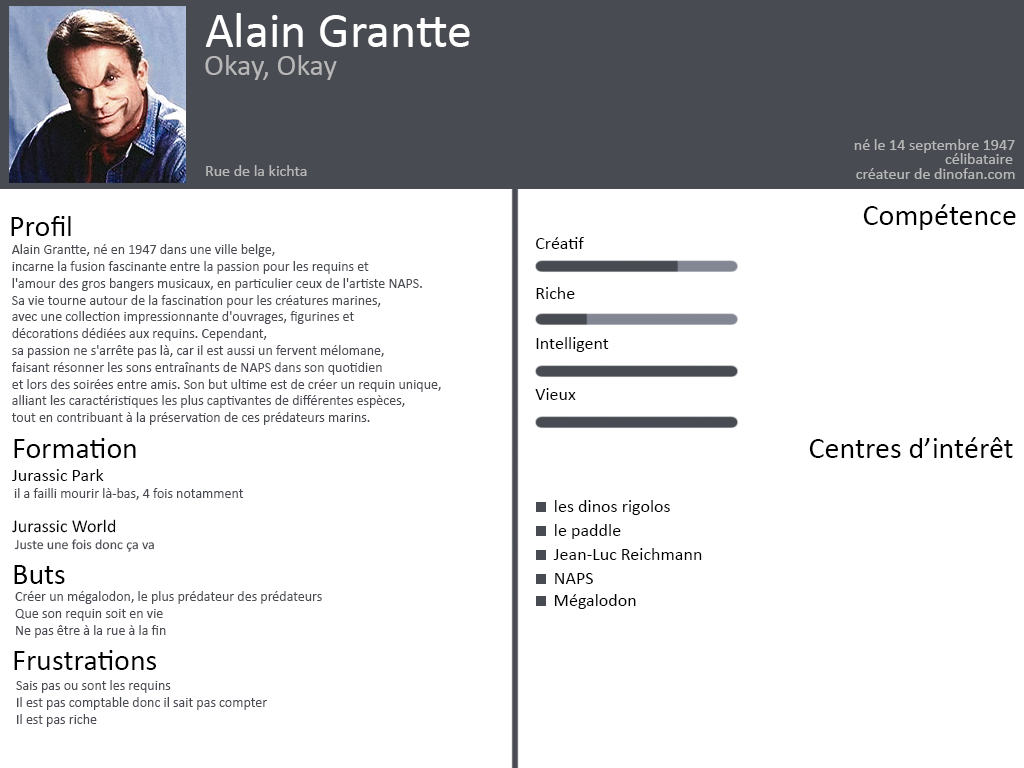
\includegraphics[width=16.4cm]{assets/persona/alain_grantte}
	\caption{\label{assets/persona/alain_grantte} Persona Alain Grantte}
\end{figure}

\newpage
\section{Abstraction des tâches}

\subsection{Description des tâches}
\begin{itemize}
    \item Étant un passionné de requin, Alan Grant décide de créer son propre requin à partir de différentes parties d'autres requins déjà existant. Comme il n'est pas un expert des requins et du milieu marin de façon générale il lui faut un outils qui l'aidera dans son projet. Alan décide donc d'utiliser l'application \textit{Pimp My Requin} pour créer son requin de rêve.
    \item Dans un premier temps, Alan peut choisir la partie du requin qu'il voudrait récupérer.
    \item Ensuite, l'utilisateur peut choisir les caractéristiques de la partie du requin sélectionné. Il peut par exemple déterminer la longueur de la nageoire de son requin.
    \item Après avoir défini les caractéristiques de la partie du requin, Alan peut comparer les différentes espèces qui respecte ses critères et établir laquelle sera la meilleur pour son propre requin. 
    \item Une fois la comparaison faite, il peut choisir l'espèce qui lui convient et l'ajouter à sa configuration, pour chaque espèce, notre outil lui donne une estimation du temps et du coût nécessaire à la création de son requin.
    \item Enfin, il a un aperçu du voyage qu'il devra effectuer pour créer son requin et il peut choisir si il veut un voyage avec une distance minimale ou un coût minimal.
\end{itemize}

\subsection{Formalisation des tâches}
\begin{enumerate}
	\item Identifier la partie du requin que l’on souhaite récupérer.
	\item Comparer les caractéristiques de la partie du requin.
	\item Consulter les espèces de requin dans le but de définir l’espèce qui permet de récupérer plusieurs parties en une fois.
	\item Synthétiser une liste d’espèces de requin qui constituera les étapes du voyage à réaliser pour finaliser le mégalodon.
	\item Dériver le voyage à réaliser pour récupérer les parties du/des différents requins.
	\item Comparer la durée et le coût du trajet afin d’optimiser la récupération de plusieurs parties de requin.
\end{enumerate}


\newpage
\section{Prototype de basse fidélité}

\begin{figure}[!h]
	\centering
	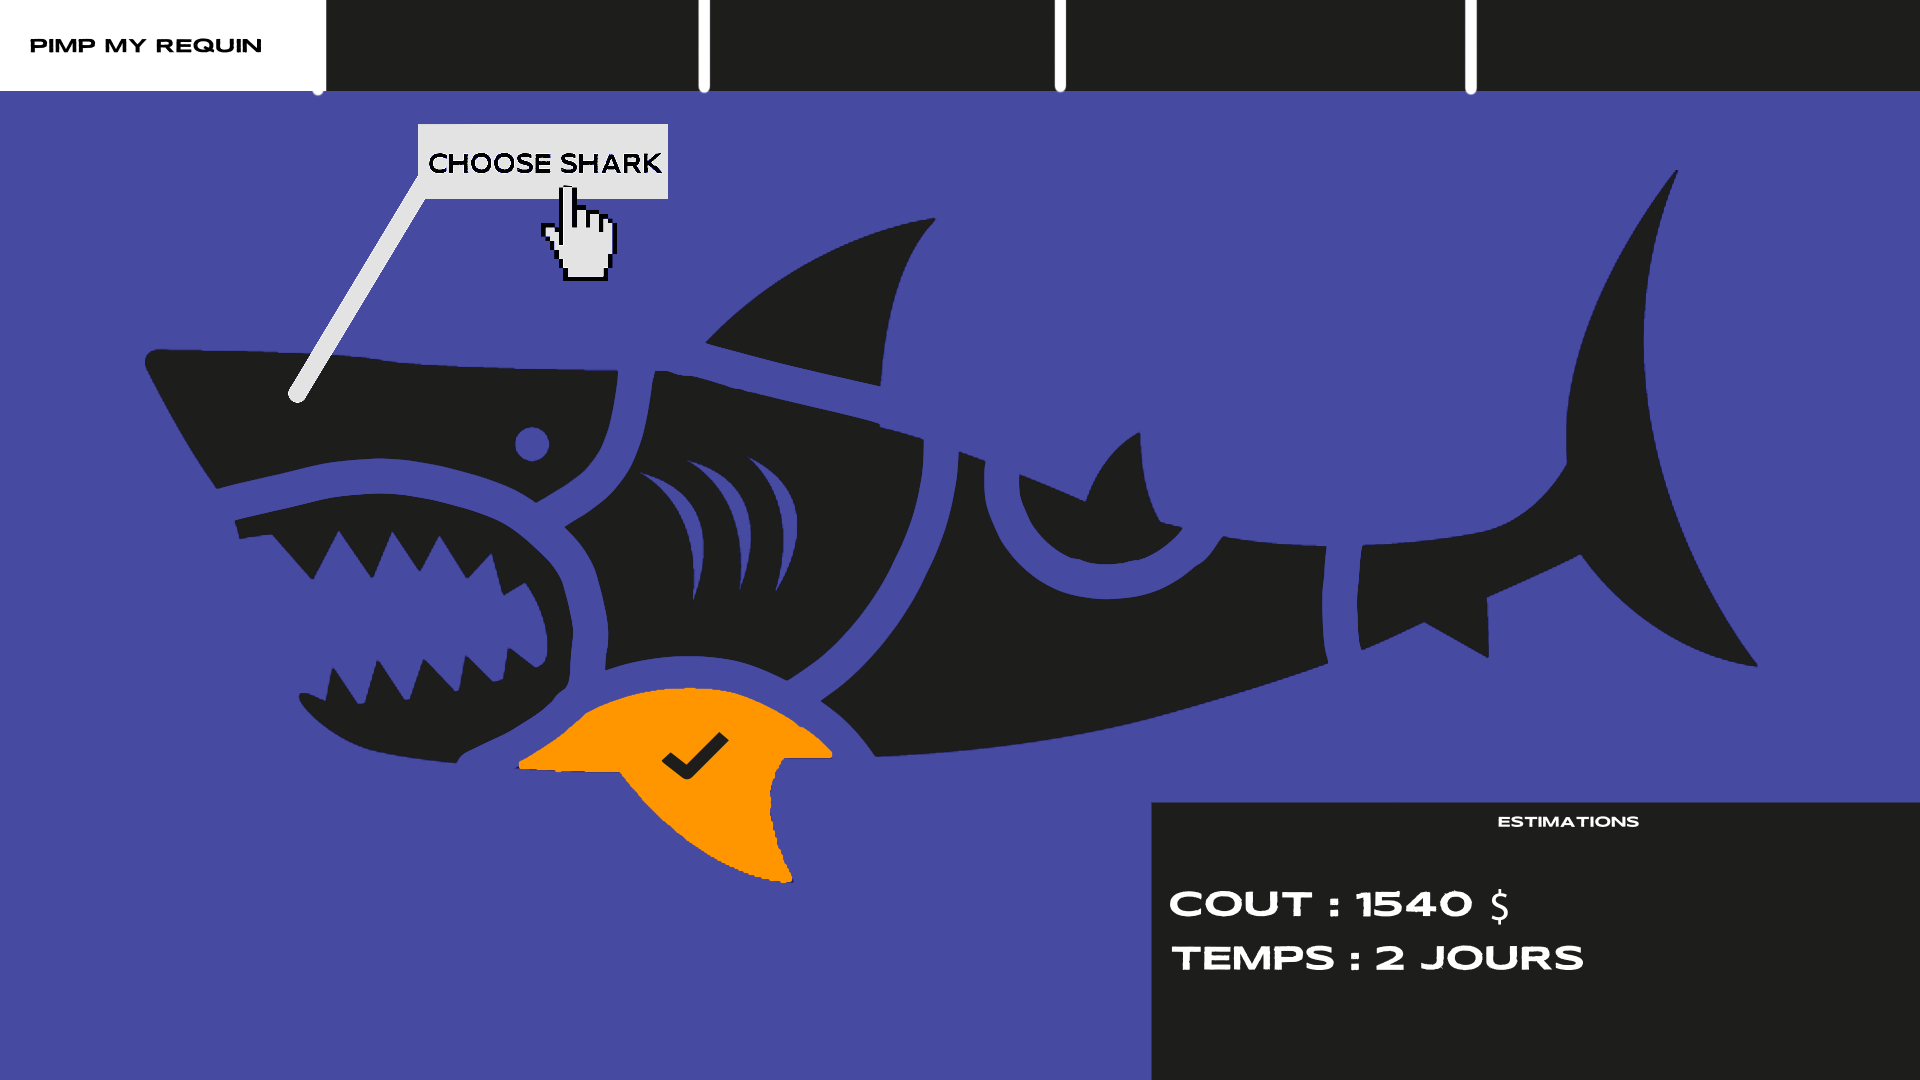
\includegraphics[width=14.4cm]{assets/prototype/basse/onglet1}
	\caption{Choix partie requin – Onglet "Pimp my requin". Permet de choisir la partie du requin que l'on veut compléter}
    \label{onglet1} 
\end{figure}

\vspace{0.3cm}

\begin{figure}[!h]
	\centering
	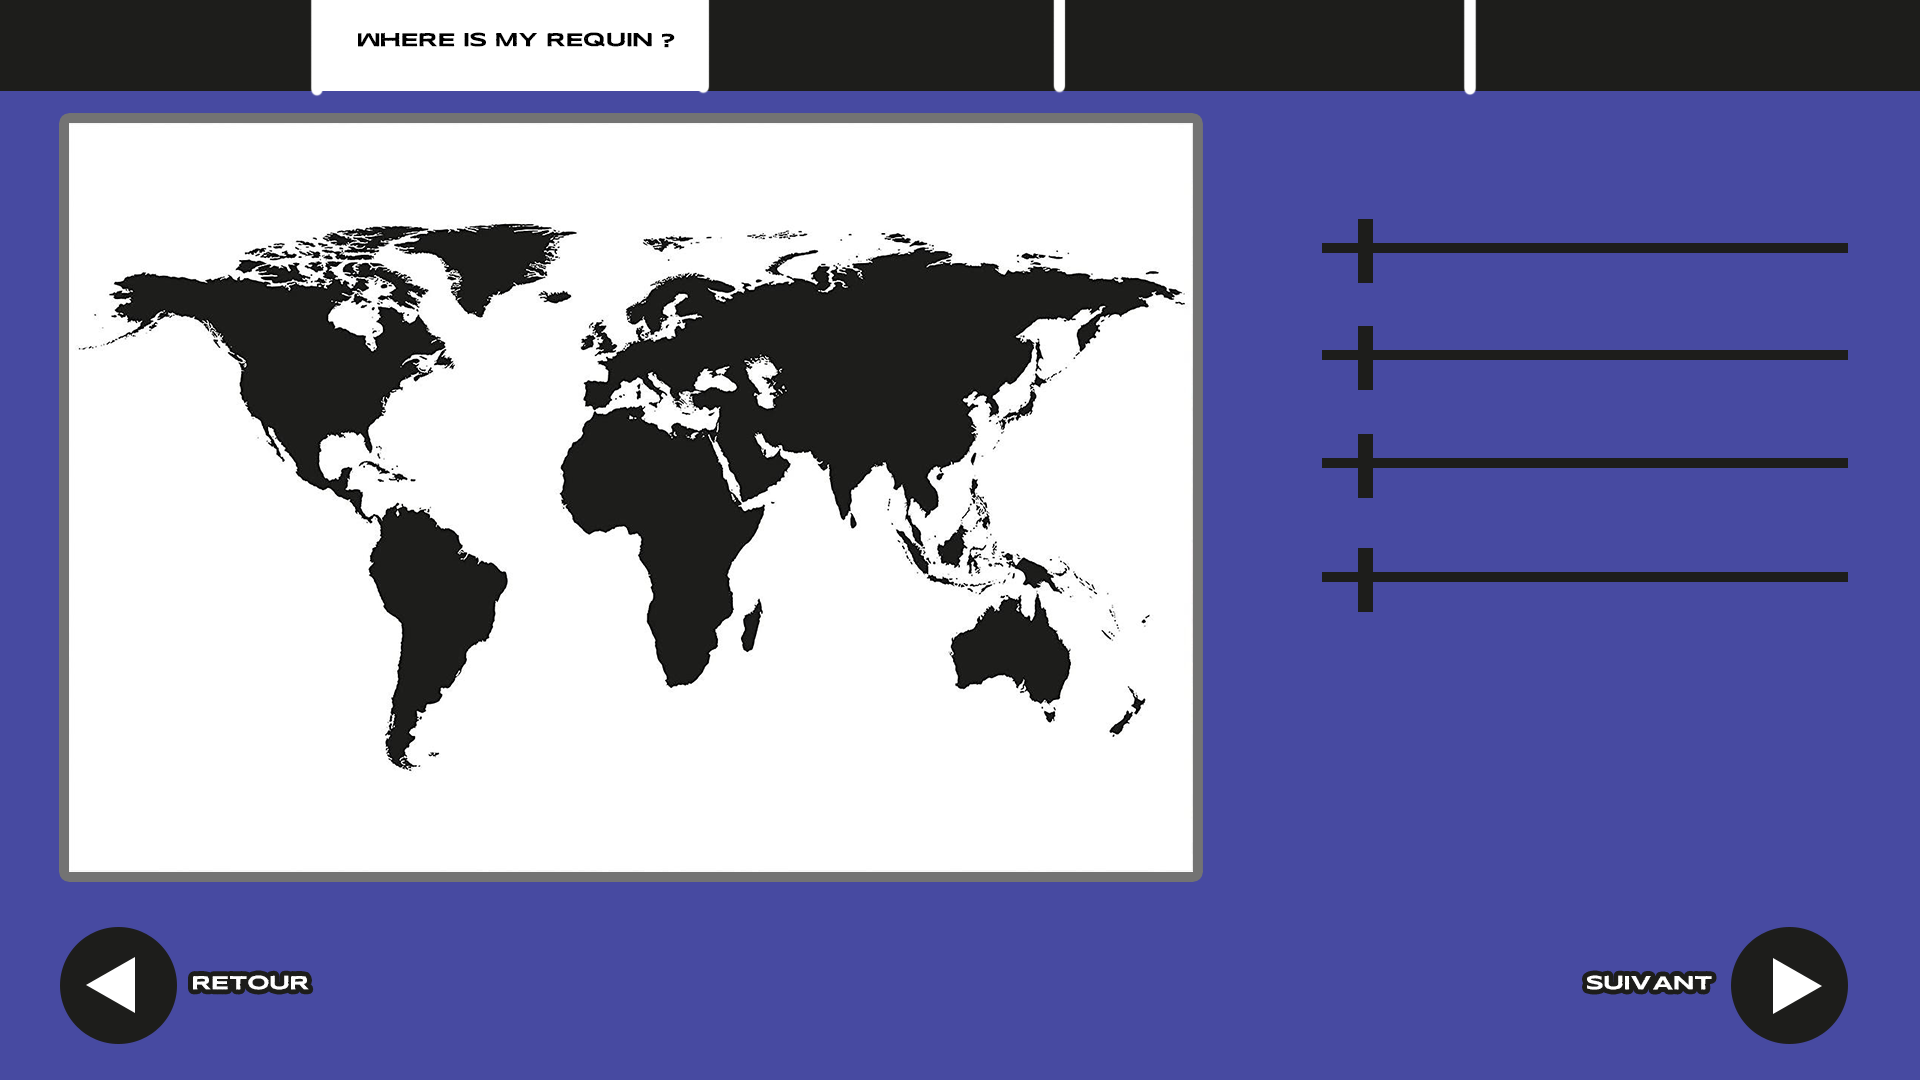
\includegraphics[width=14.4cm]{assets/prototype/basse/onglet2}
	\caption{ Choix caractéristique – Onglet "Where is my requin ? Permet de filtrer les requins selon nos besoins a l'aide des caractéristiques"}
    \label{onglet2}
\end{figure}

\begin{figure}[!h]
	\centering
	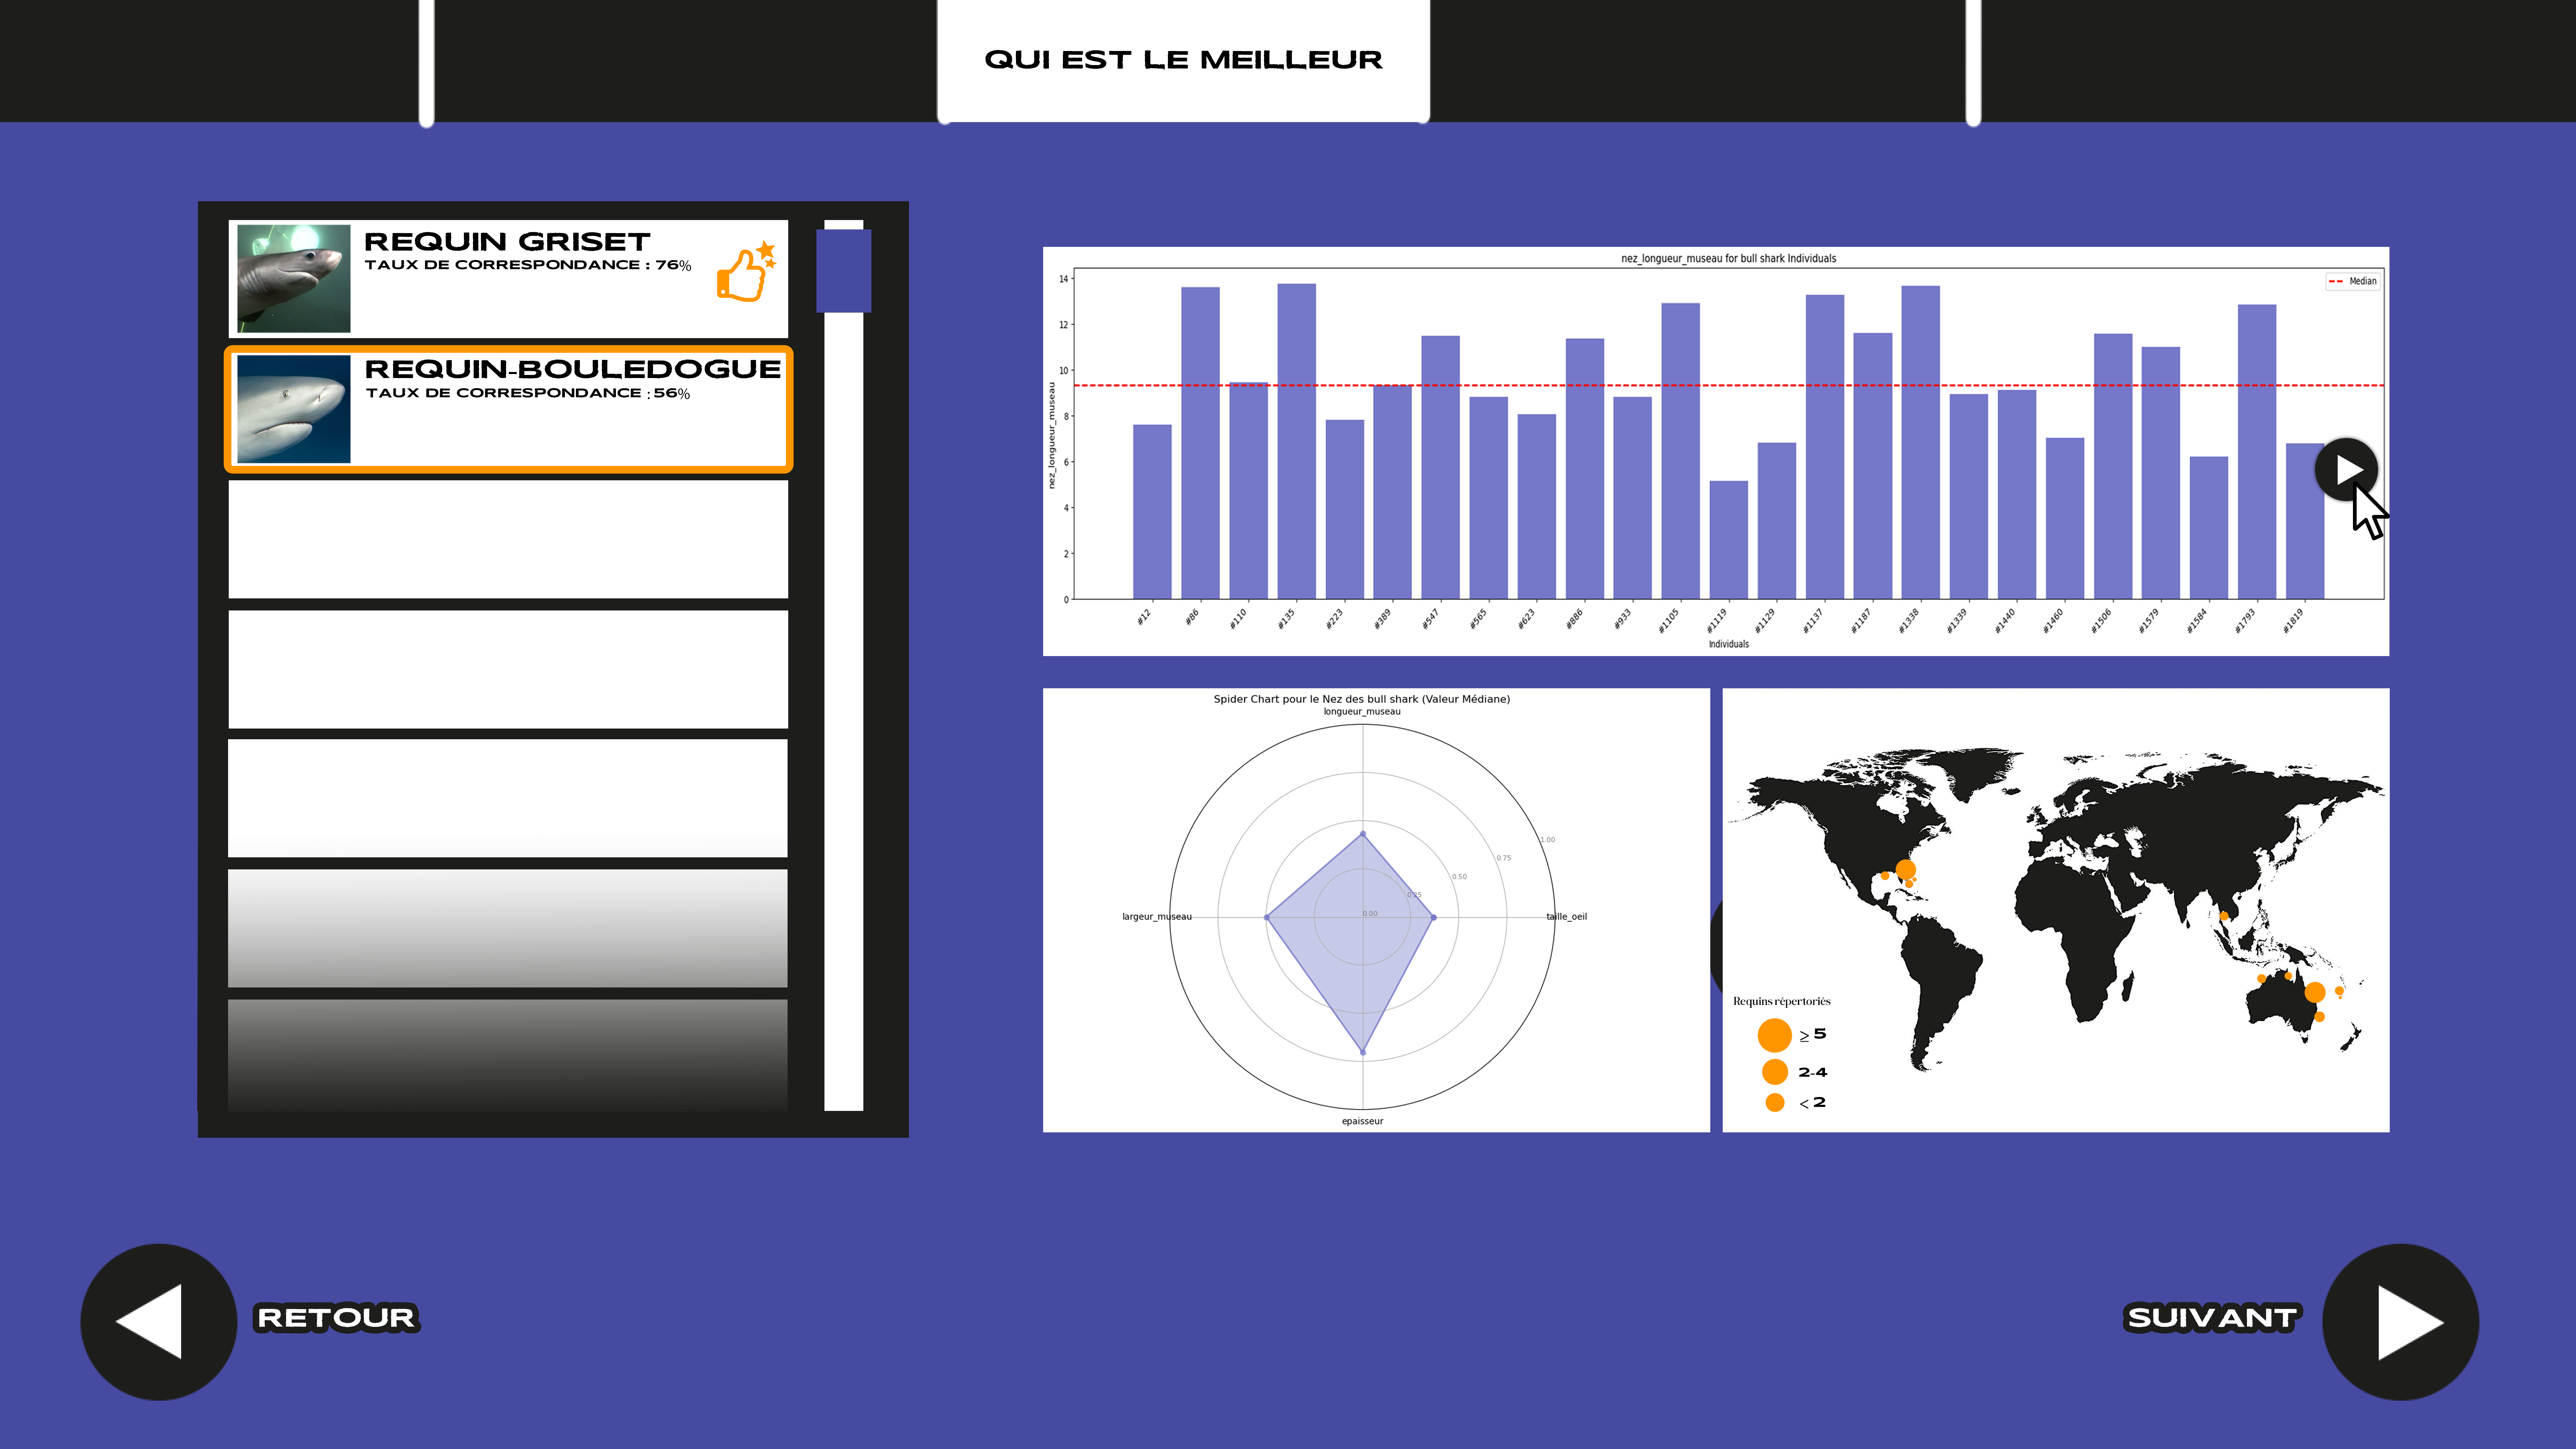
\includegraphics[width=14.4cm]{assets/prototype/basse/onglet3}
	\caption{ Comparaison des espèces vis-à-vis de leurs caractéristiques – Onglet "Who's da best". Permet de comparer les espèces entre-elles via des bar-chart, un spider-chart et une carte montrant ou trouver cette espèce.}
    \label{onglet3}
\end{figure}

\vspace{1cm}

\begin{figure}[!h]
	\centering
	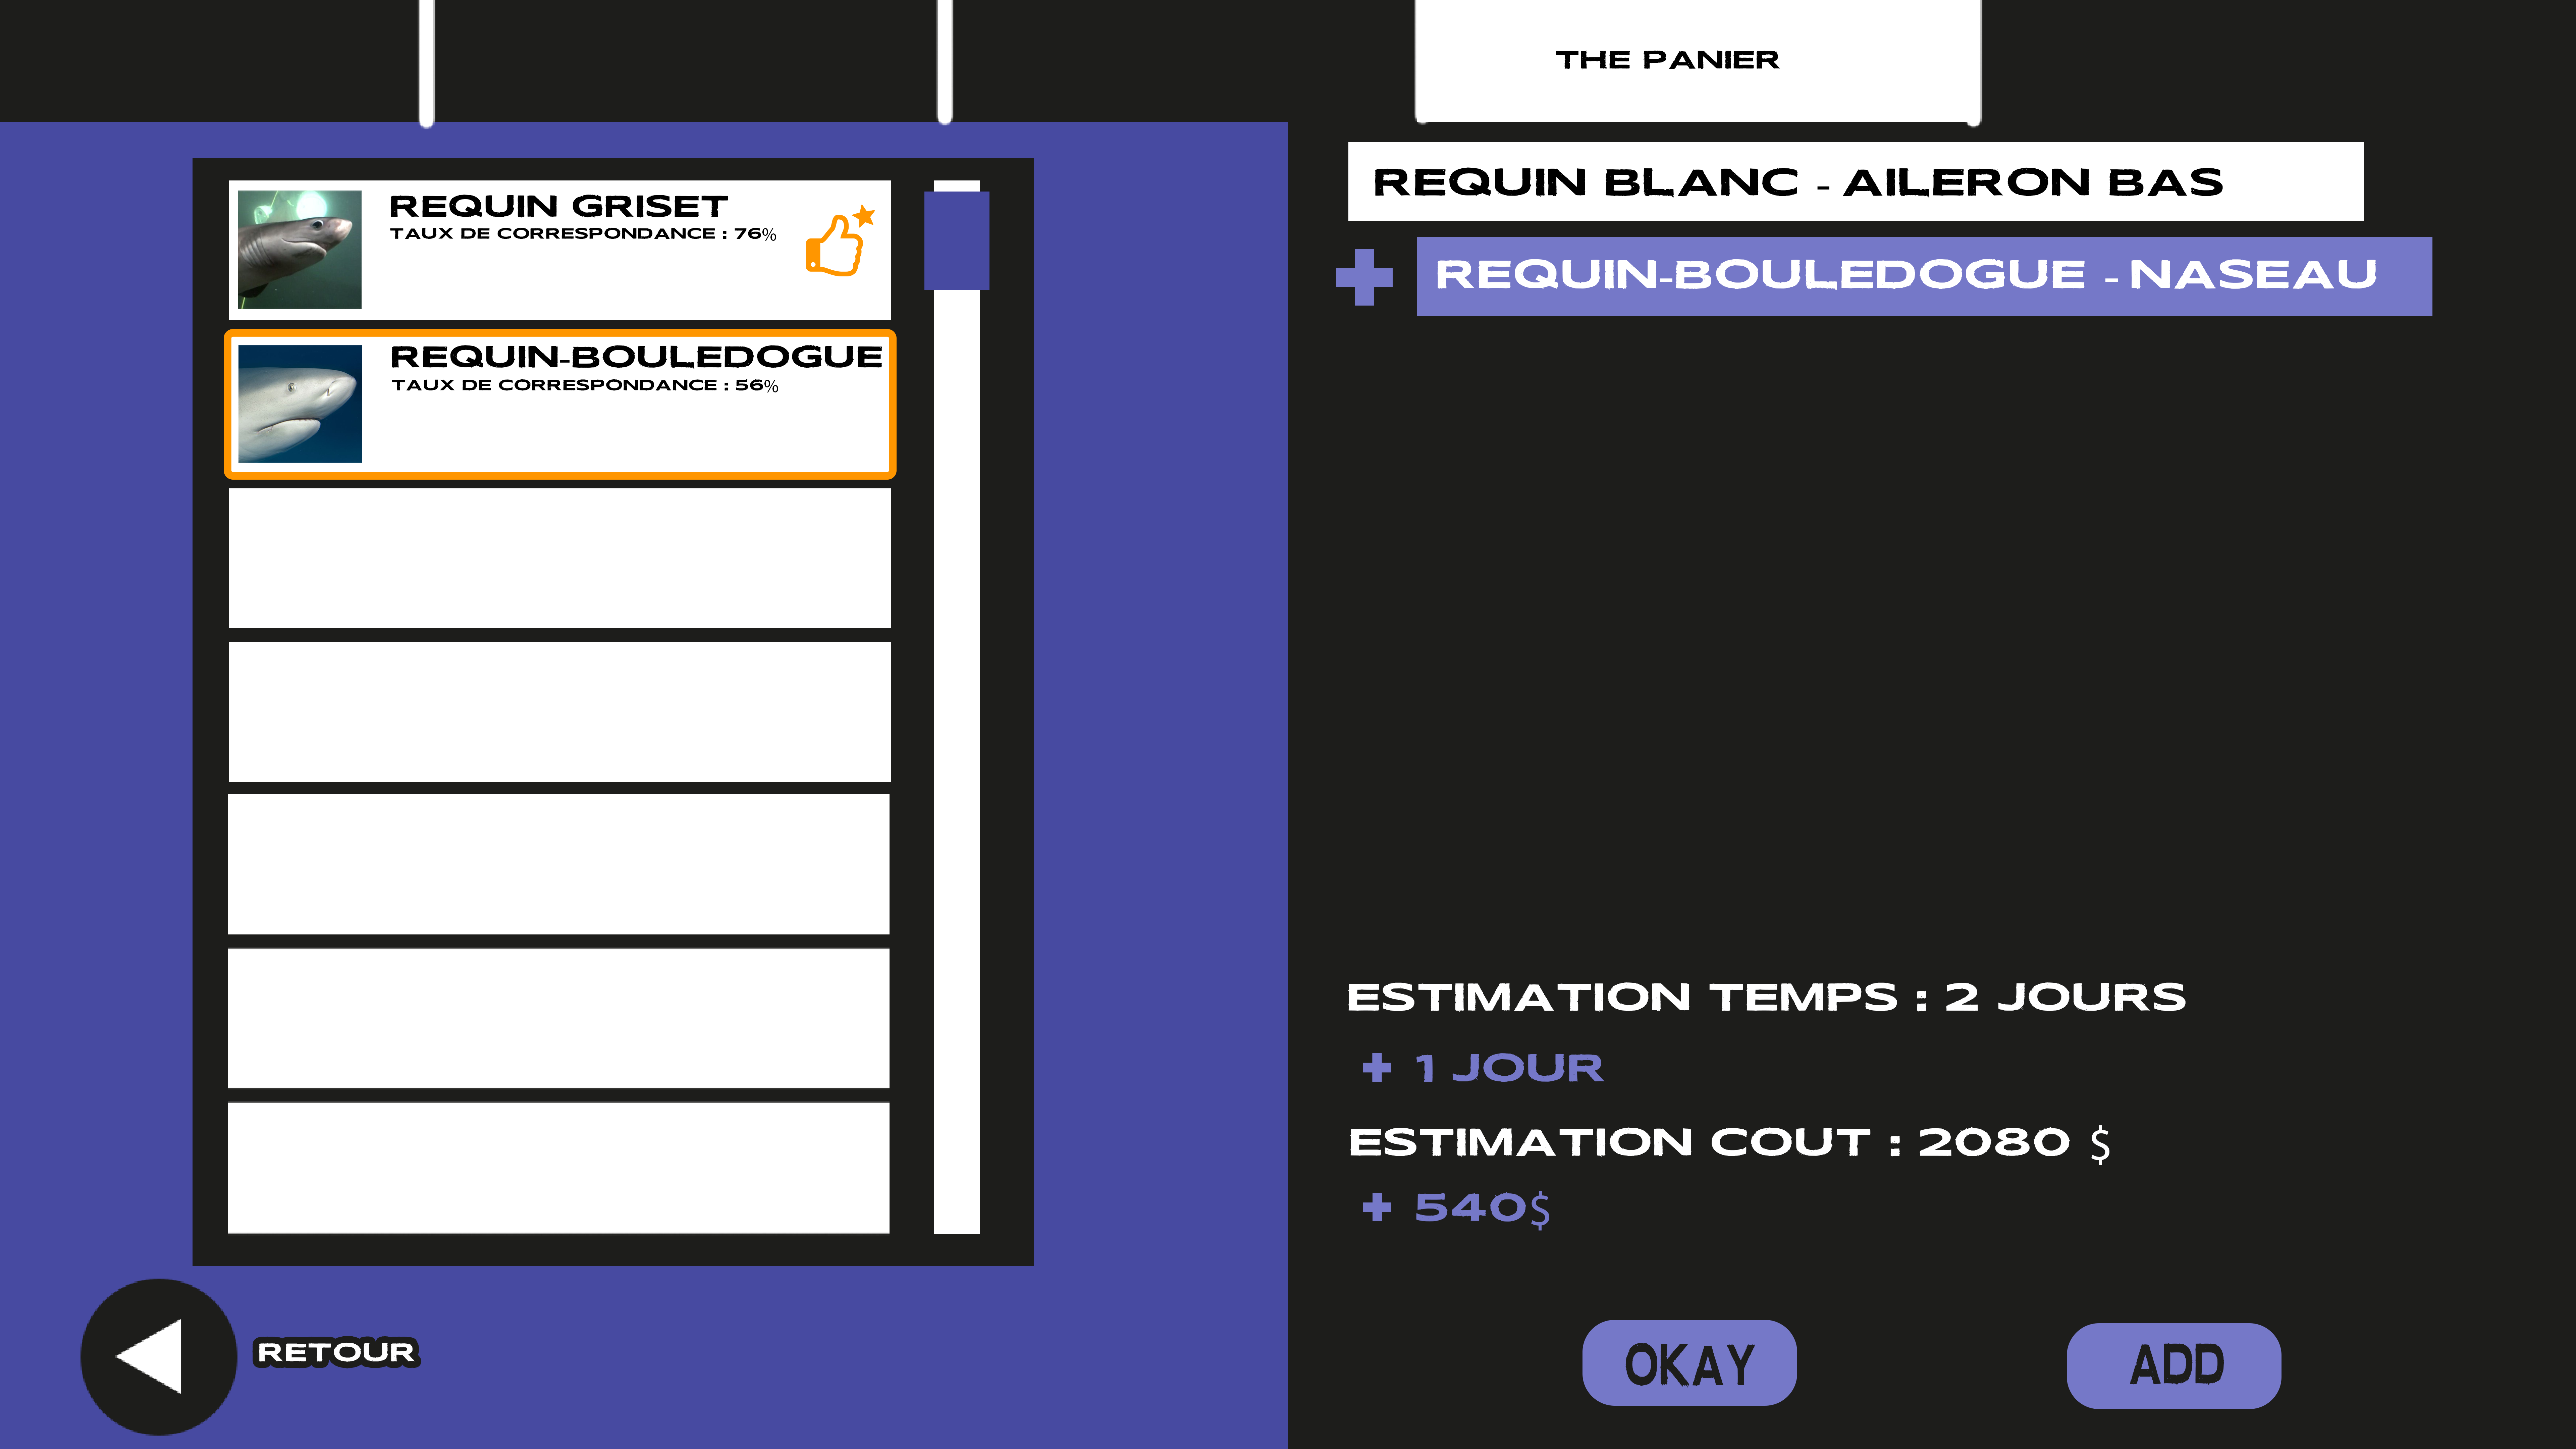
\includegraphics[width=14.4cm]{assets/prototype/basse/onglet4}
	\caption{Établir un panier d’espèce de requin – Onglet "The panier". Permet de voir les requins déja choisi avec le possible candidat afin de déterminer l'impact du cout et du temps.}
    \label{onglet4} 
\end{figure}

\begin{figure}[!h]
	\centering
	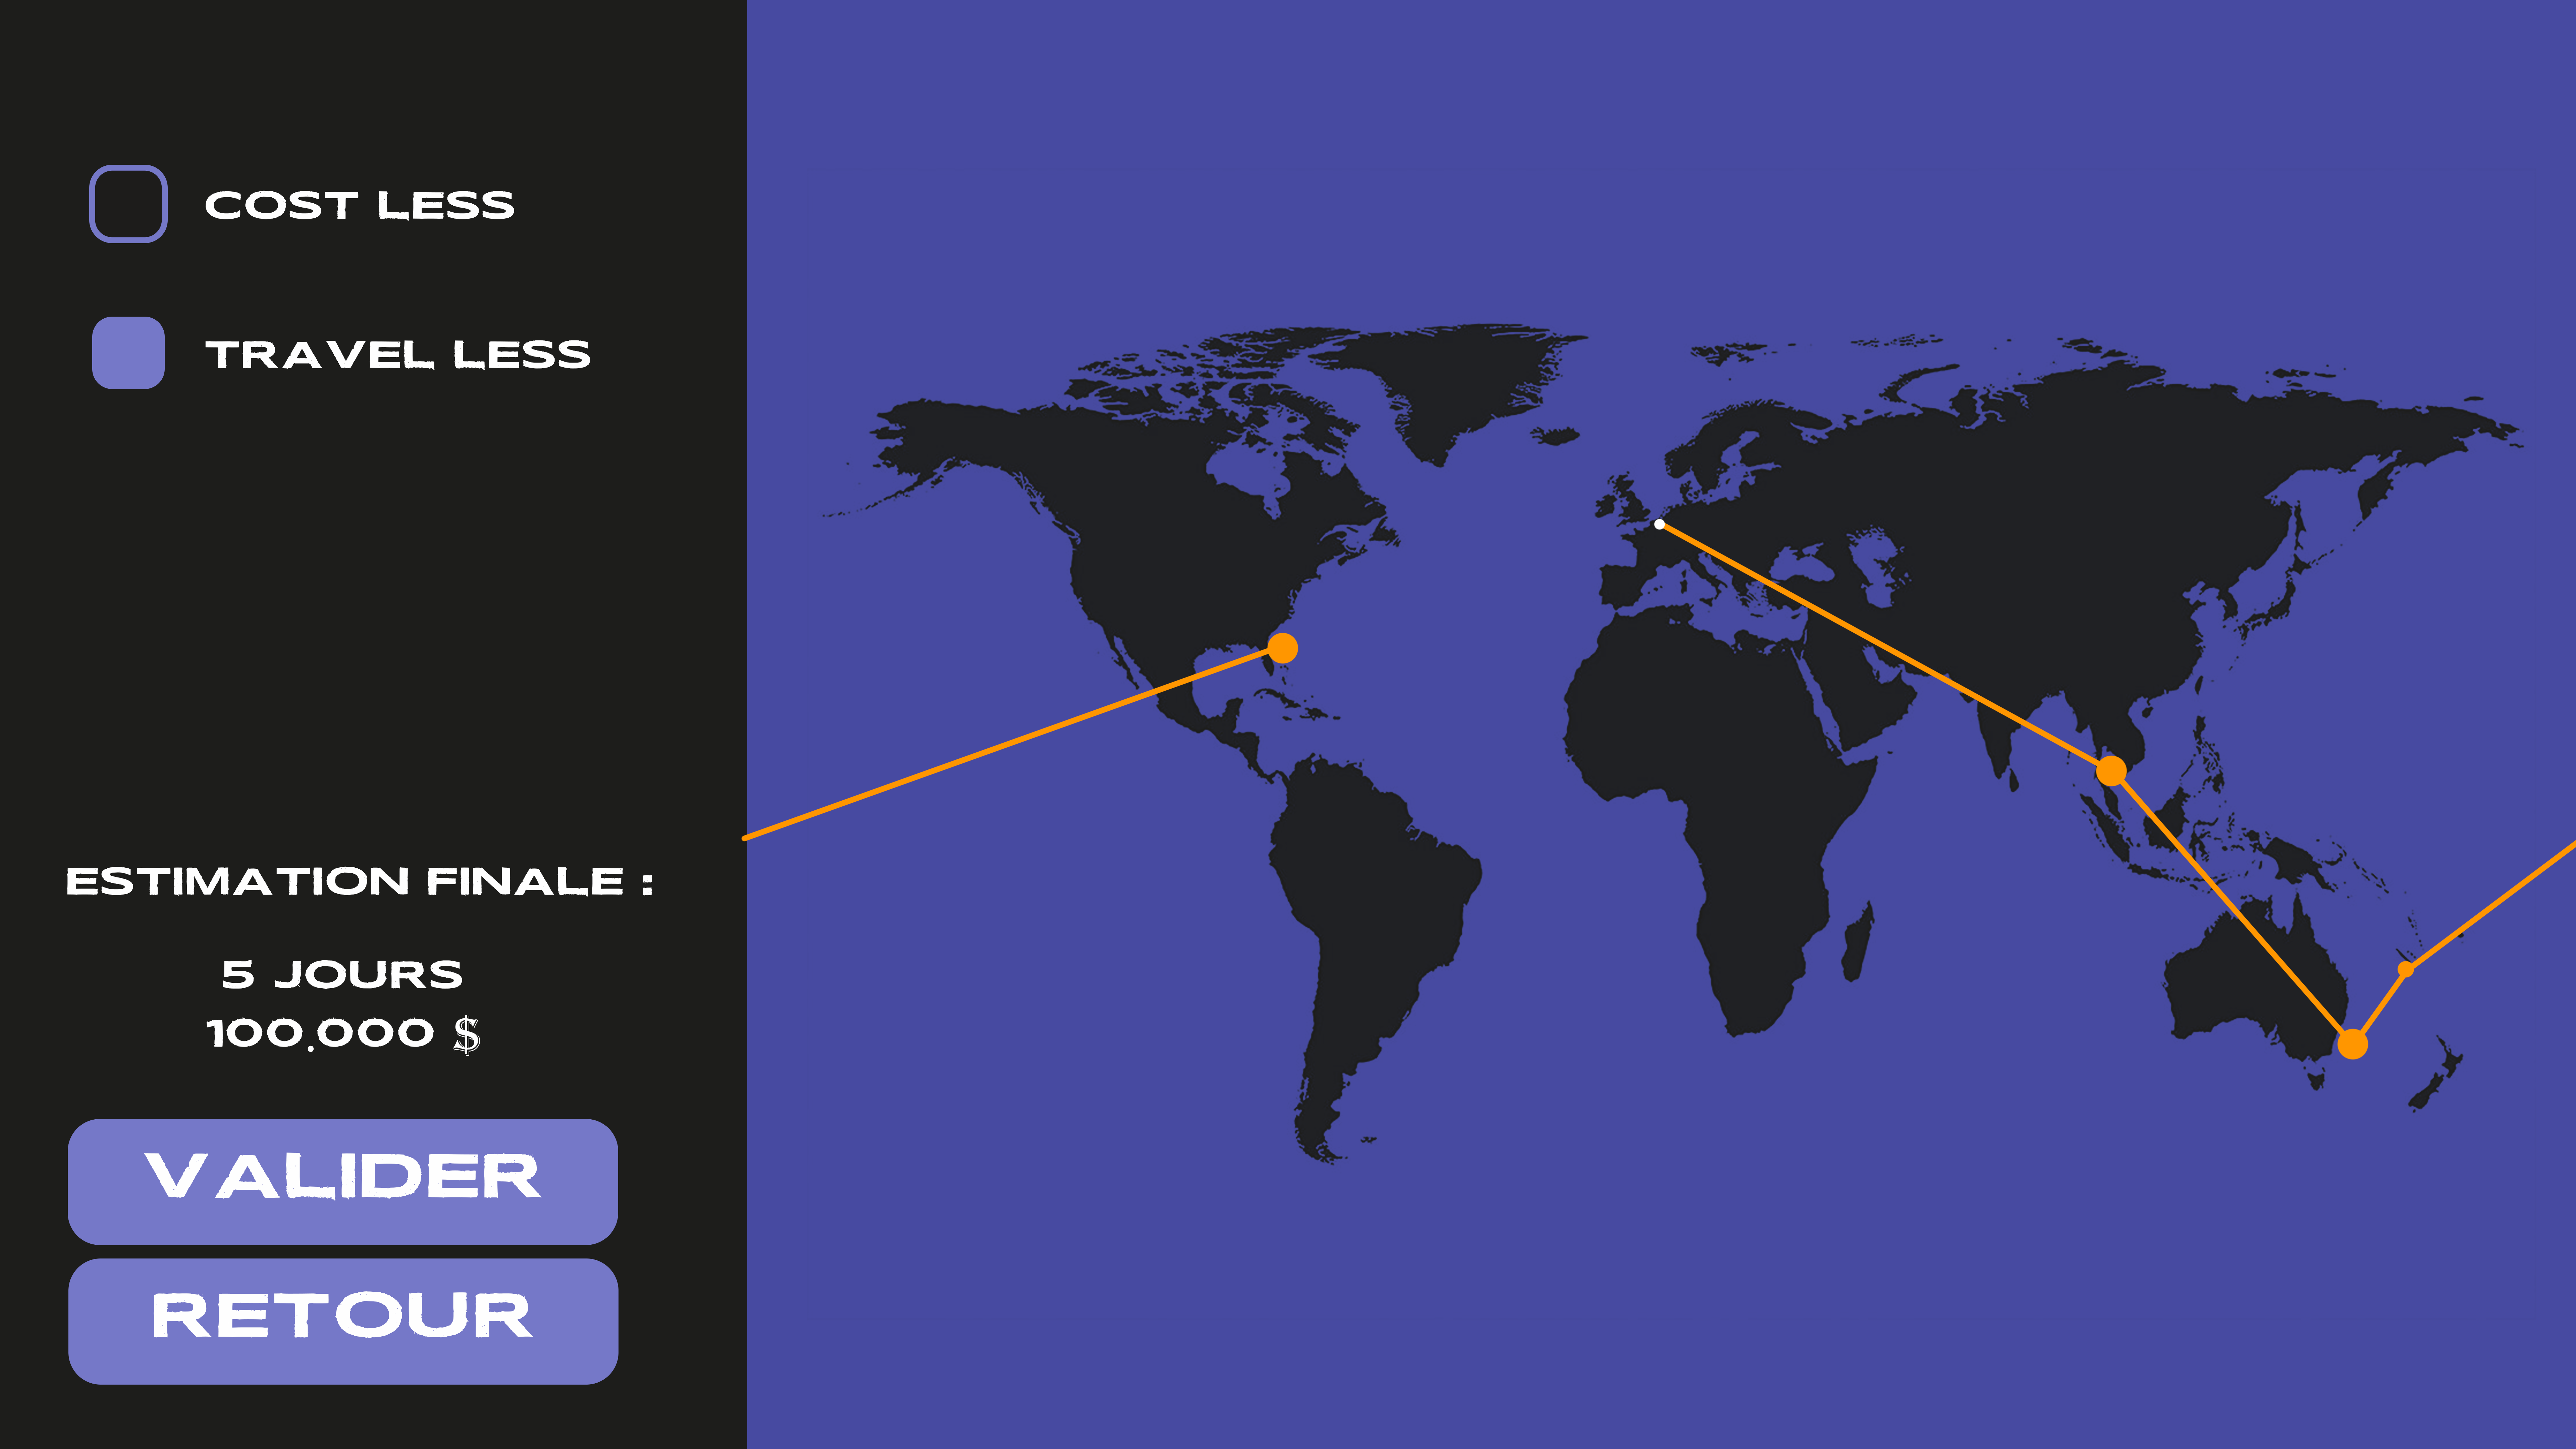
\includegraphics[width=14.4cm]{assets/prototype/basse/onglet5}
	\caption{Visualisation du voyage.}
    \label{onglet5} 
\end{figure}

\clearpage
\section{Mapping entre les tâches et le prototype}


\begin{center}
	\begin{tabular}{|p{3.5cm}|p{7cm}|p{3.5cm}|}
		\hline
		Tâches
		&
		Explications
		&
		Figures
		\\\hline
		1. Identifier la partie du requin que l’on souhaite récupérer.
		&
		Ce choix se fera via le schéma du requin en milieu de page.
		&
        
		Figure \ref{onglet1} – Choix partie requin – Onglet "Pimp my requin".
		\\\hline
		2. Comparer les caractéristiques de la partie du requin.
		&
		Définir les caractéristiques se fera via les différents "sliders" (curseurs) présent sur la droite de la page.
		&
		Figure \ref{onglet2} – Choix caractéristique – Onglet "Where is my requin ?".
		\\\hline
		3. Consulter les espèces de requin dans le but de définir l’espèce qui permet de récupérer plusieurs parties en une fois.
		&
		Il sera possible de déterminer l’espèce de requin que l’on souhaite visualiser via la liste présente sur la gauche de la page. Une fois le choix de l’espèce effectué, les différentes visualisations sur la droite de la page s'actualisent. Un Bar Chart pour chacunes des caractéristiques nous montrerons la fluctuations de cette dernière à travers l'espèce, Nous aurons aussi un Spider Chart afin de voir plus directement si l'espèce choisie coche plusieurs des cases de l'utilisateur. Ensuite, une petite carte montrera où cette espèce à été apperçue dernièrement. De plus, dès qu'il est possible de regrouper des parties via une seule espèce, l'espèce permettant cela sera mise en avant par un petit logo "recommandation".
		&
		Figure \ref{onglet3} – Comparaison des espèces vis-à-vis de leurs caractéristiques – Onglet "Who's da best".
		\\\hline
		4. Synthétiser une liste d’espèces de requin qui constituera les étapes du voyage à réaliser pour finaliser le mégalodon.
		&
		Sur cette page, la partie gauche sera dédiée à la liste des différentes espèces de requin. Tandis que la droite sera dédiée au "panier" auquel sera ajoutée l’espèce que l’on souhaite. Cette page sera sauvegardée jusqu’à la validation du voyage. Un bouton "add" permet de revenir à la première page (Figure 1) et permettra de recommencer le processus avec une partie que l’on n'a pas encore sélectionnée par le passé.
		&
		Figure \ref{onglet4} – Établir un panier d’espèce de requin – Onglet "The panier".
		\\\hline
		5. Dériver le voyage à réaliser pour récupérer les parties du/des différents requins.
		&
		La visualisation du voyage se fera sur la carte en milieu de page.
		&
		Figure \ref{onglet5} – Visualisation du voyage.
		\\\hline
		6. Comparer la durée et le coût du trajet afin d’optimiser la récupération de plusieurs parties de requins.
		&
		La comparaison sera possible via les différentes à cocher sur la gauche de la page. Une case montrera le voyage avec le coût le plus faible et l’autre case montrera le voyage le moins coûteux en temps.
		&
		Figure \ref{onglet5} – Visualisation du voyage.
		\\\hline
	\end{tabular}
\end{center}

\section{Protocole d'évaluation}
Dans cette partie, nous allons décrire notre protocole d’évaluation. Nous avons décidé d'opter pour une approches qualitative car tout les scientifiques ne souhaitent pas créer des requins.

\subsection{Test utilisateur}

\subsubsection{Objectifs}
L'objectif principal de notre test utilisateurs est l'évaluation de l'interface de notre solution. En effet, nous estimons avoir une solution suffisamment fonctionnelle qui permet de simuler certaines taches d'exécution. 
Notre attention se porte particulièrement sur l'évaluation de la convivialité de notre outil de visualisation, tout en veillant à identifier tout problème éventuel lors de la séquence d'exécution des tâches.
 a

\subsubsection{Scénarios}

\paragraph{Scénario 1 : Créer un requin librement}
Informations données à l'utilisateur :
\begin{itemize}
    \item Vous allez assembler un requin en combinant des parties prélevées sur différents requins.
    \item Chaque composant doit provenir d'un requin que vous avez sélectionné.
\end{itemize}

Aide pour les commentaires de la grille d'évaluation :
\begin{itemize}
    \item Quelle était la première action réalisée ?
    \item Quelle partie du requin avez-vous choisie en premier ?
\end{itemize}

\paragraph{Scénario 2 : Créer le requin le plus grand possible}
Informations données à l'utilisateur :
\begin{itemize}
    \item Vous allez assembler un requin en combinant des parties prélevées sur différents requins en ayant les plus grandes caractéristiques possibles.
    \item Chaque composant doit provenir d'un requin que vous avez sélectionné.
    \item Les filtres vous permettent d'obtenir une taille minimale.
    \item La carte vous montre s'il existe des espèces par rapport à vos filtres.
\end{itemize}

Aide pour les commentaires de la grille d'évaluation :
\begin{itemize}
    \item Quelle était la première action réalisée ?
    \item Quelle espèce de requin avez-vous choisie en premier ?
\end{itemize}

\paragraph{Scénario 3 : Créer le requin le plus grand possible sans bouger de l'Europe}
Informations données à l'utilisateur :
\begin{itemize}
    \item Vous allez assembler un requin en combinant des parties prélevées sur différents requins en ayant les plus grandes caractéristiques possibles.
    \item Chaque composant doit provenir d'un requin venant d'Europe.
    \item Les filtres vous permettent d'obtenir une taille minimale.
    \item La carte vous montre s'il existe des espèces par rapport à vos filtres.
    \item L'onglet final doit être seulement composé de points se trouvant en Europe.
\end{itemize}

Aide pour les commentaires de la grille d'évaluation :
\begin{itemize}
    \item Quelle était la première action réalisée ?
    \item Quel est le coût total et le nombre de voyages finaux ?
\end{itemize}

\paragraph{Scénario 4 : Créer un requin avec un minimum de 3 voyages}
Informations données à l'utilisateur :
\begin{itemize}
    \item Vous allez assembler un requin en combinant des parties prélevées sur différents requins.
    \item Chaque composant doit provenir de requins qui se trouve au minimum à 3 endroits différents.
    \item Les filtres vous permettent d'obtenir une taille minimale.
    \item La carte vous montre s'il existe des espèces par rapport à vos filtres.
    \item L'onglet final doit être composé de 3 voyages minimum.
\end{itemize}

Aide pour les commentaires de la grille d'évaluation :
\begin{itemize}
    \item Quelle était la première action réalisée ?
    \item Quel est le coût total et le nombre de voyages finaux ?
\end{itemize}

\paragraph{Scénario 5 : Créer un requin avec un maximum de 10000 dollars}
Informations données à l'utilisateur :
\begin{itemize}
    \item Vous allez assembler un requin en combinant des parties prélevées sur différents requins.
    \item Le montant total pour votre requin ne doit pas dépasser 10000 dollars.
    \item Les filtres vous permettent d'obtenir une taille minimale.
    \item La carte vous montre s'il existe des espèces par rapport à vos filtres.
    \item Le premier et dernier onglet vous montrent l'estimation du coût.
\end{itemize}

Aide pour les commentaires de la grille d'évaluation :
\begin{itemize}
    \item Quelle était la première action réalisée ?
    \item Quel est le coût total ?
    \item Quel est le nombre d'espèces différentes qui composent votre requin ?
\end{itemize}

\paragraph{Scénario 6 : Créer un requin avec un maximum de 5000 dollars et 2 voyages}
Informations données à l'utilisateur :
\begin{itemize}
    \item Vous allez assembler un requin en combinant des parties prélevées sur différents requins.
    \item Le montant total pour votre requin ne doit pas dépasser 5000 dollars.
    \item Vous n'avez droit qu'à 2 voyages.
    \item Les filtres vous permettent d'obtenir une taille minimale.
    \item La carte vous montre s'il existe des espèces par rapport à vos filtres.
    \item Le premier et dernier onglet vous montrent l'estimation du coût.
\end{itemize}

Aide pour les commentaires de la grille d'évaluation :
\begin{itemize}
    \item Quelle était la première action réalisée ?
    \item Est-ce possible ?
    \item Si oui, quel est le nombre d'espèces différentes qui composent votre requin ?
    \item Quel est le coût total et le nombre de voyages finaux ?
\end{itemize}

\subsubsection{Grille d'observation}

\begin{table}[h]
\centering
\begin{tabular}{|p{6cm}|p{1.5cm}|p{1.5cm}|p{2.5cm}|p{3.5cm}|}
\hline
Scénario & Durée & Actions & Problèmes rencontrés et sources & Commentaires \\ \hline
1. Créer un requin librement & ... & ... & ... & ... \\ \hline
2. Créer le requin le plus grand possible & ... & ... & ... & ... \\ \hline
... & ... & ... & ... & ... \\ \hline
6. Créer un requin avec un maximum de 5000 dollars et 2 voyages & ... & ... & ... & ... \\ \hline
\end{tabular}
\end{table}

\begin{table}[h]
\centering
\begin{tabular}{|p{4cm}|p{6cm}|}
\hline
L’utilisateur va-t-il tenter d’effectuer l’action appropriée?  &  Non (1) O O O O O Oui (5)\\ \hline
L’utilisateur saura-t-il que l’action appropriée est disponible?  &  Non (1) O O O O O Oui (5)\\ \hline
L’utilisateur associera-t-il l’effet désiré à l’action appropriée?  &  Non (1) O O O O O Oui (5)\\ \hline
Si l’action appropriée est effectuée, l’utilisateur se rendra-t-il compte qu’il progresse vers son objectif?  &  Non (1) O O O O O Oui (5)\\ \hline
\end{tabular}
\end{table}

\begin{table}[h]
\centering
\begin{tabular}{|p{10cm}|}
\hline
Recommandation  \\ \hline
...  \\ \hline
\end{tabular}
\end{table}

\clearpage
\subsubsection{Recrutement des utilisateurs}
Nous prévoyons de recruter cinq utilisateurs, en particulier des paléontologues ayant une expertise certaines dans l'anatomie sous-marine des animaux. Nous souhaitons également inclure des paléontologues qui ont de l'expérience dans les parcs "Jurassic Park" et "Jurassic World", car leurs expériences pourraient nous fournir des informations précieuses sur la faisabilité de recréer un Mégalodon.



\subsubsection{Passation}
La passation du test se fera dans une salle qui inspire le comfort, de sorte à ce que les seules frustrations possibles viennent de notre outil. Les observateurs posséderont une suite d'actions pour chaque scénarios. Pour chaque test, il y aura un utilisateur et 3 observateur. Les tests seront enregistrés, à la fois l'interface et l'utilisateur.

C'est pour cela qu'avant de commencer les tests, les utilisateurs devront signer le formulaire de consentement certifié conforme au RGPD. Après avoir expliqué brièvement le but de l'application, l'utilisateur prendra part au différents scénarios et nous appliquerons la technique "Think Aloud" pour que nous puissions en prendre notes.
Les observateurs noteront toute déviations par rapport à la suite d'actions "optimales"

Un court débriefing se tiendra avant le départ des utilisateurs dans lequel nous poserons ces questions : 
" Y'a t-il une étape qui vous a ralenti ? Si oui pourquoi ?"
" Avez vous eu des problèmes pour bien sélectionner vos espèces de requins?"
\subsection{Type d'évaluation}
Nous avons décidé d'utiliser l'inspection cognitive car cela répondait au mieux à ce que nous souhaitions faire. Nous essayons de ce fait d'appliquer au mieux cette méthodologie d'évaluation. Grâce à cela, nous espérons déterminer si notre interface est suffisamment claire, si ce n'est pas le cas, nous verrons assez simplement les parties qui demande un changement.

\end{document}